\section{Integral}
\begin{frame}{Antiderivatives}
    \begin{block}{Definition}
        A function \textit{F} is called an antiderivative of \textit{f} on an interval \textit{I} if \textit{F'(x) = f(x)} for all \textit{x} in \textit{I}.
    \end{block}
    \begin{block}{Theorem}
        If \textit{F} is an antiderivative of \textit{f} on an interval \textit{I}, then the most general antiderivative of \textit{f} on \textit{I} is $$F(x)+C$$,
        where C is an arbitrary constant.
    \end{block}
    \begin{center}
        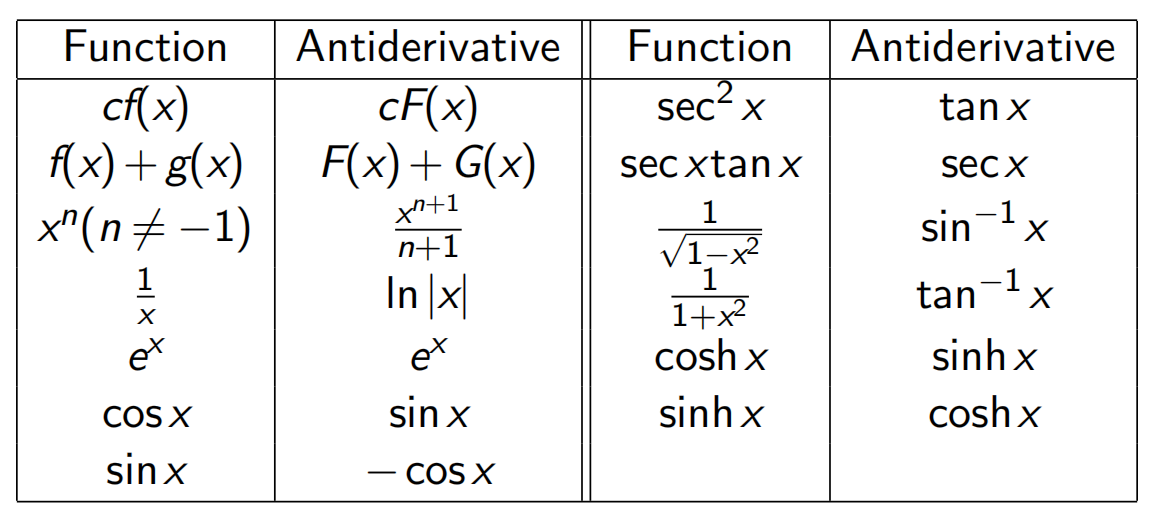
\includegraphics[height=3cm]{res/anti.png}
    \end{center}

\end{frame}

\begin{frame}{Antiderivatives}
    \begin{block}{notation}
        $$
            \int f(x) d x=F(x) \quad \text { means } \quad F^{\prime}(x)=f(x)
        $$
    \end{block}
    How to understand this notation?
    \begin{block}{Theorem}
        If the antiderivatives of functions \textit{f(x)} and \textit{g(x)} exist, then for any constant \textit{p} and \textit{q}, the antiderivate of \textit{pf(x)+qg(x)} also exists, and we have
        $$\int[pf(x)+qg(x)]dx=p\int f(x)dx+q\int g(x)dx$$
    \end{block}
\end{frame}

\begin{frame}{Indefinite Integrals}
    Keep the following indefinite integrals firmly in mind!\\
    $$
        \begin{array}{ll}
            \int c f(x) d x=c \int f(x) d x         & \int[f(x)+g(x)] d x=\int f(x) d x+\int g(x) d x \\
            \int k d x=k x+C                        & \int \dfrac{1}{x} d x=\ln \alert{|}x\alert{|}+C \\
            \int x^{n} d x=\dfrac{x^{n+1}}{n+1}+C   & \int a^{x} d x=\dfrac{a^{x}}{\ln a}+C           \\
            \int e^{x} d x=e^{x}+C                  & \int \cos x d x=\sin x+C                        \\
            \int \sin x d x=-\cos x+C               & \int \csc ^{2} x d x=-\cot x+C                  \\
            \int \sec ^{2} x d x=\tan x+C           & \int \csc x \cot x d x=-\csc x+C                \\
            \int \sec x \tan x d x=\sec x+C         & \int \dfrac{1}{\sqrt{1-x^{2}}} d x=\arcsin x+C  \\
            \int \dfrac{1}{x^{2}+1} d x=\arctan x+C & \int \cosh x d x=\sinh x+C                      \\
            \int \sinh x d x=\cosh x+C
        \end{array}
    $$
\end{frame}

\begin{frame}{Substitution Rule}
    \begin{block}{Definition}
        $$
            \int f(x) g^{\prime}(x) dx= \int f(x)dg(x)
        $$
    \end{block}
    How to memorize?\\
    $\dfrac{dg(x)}{dx}=g^{\prime}(x)$\\$\Rightarrow dx=\dfrac{dg(x)}{g^{\prime}(x)}$\\$\Rightarrow \int f(x) g^{\prime}(x) dx= \int f(x)g^{\prime}(x)\cdot \dfrac{dg(x)}{g^{\prime}(x)}=\int f(x)dg(x)$
\end{frame}

\begin{frame}{Substitution Rule}
    Type 1: Direct Substitution ($u=g(x)$)
    \begin{block}{Substitution Rule for Direct Substitution}
        If $u=g(x)$ is a differentiable function whose range is an interval $I$ and $f$ is continuous on $I$, then
        $$
            \int f(g(x)) g^{\prime}(x) dx= \int f(g(x))dg(x)=\int f(u) d u=F(u)+C
        $$
    \end{block}
    Type 2: Inverse Substitution ($x=\varphi(t)$)
    \begin{block}{Substitution Rule for Inverse Substitution}
        If $x=\varphi(t)$ is an invertible function, then
        $$
            \int f(x)dx = \int f(\varphi (t))d\varphi (t)=\int f(\varphi (t))\varphi ^{\prime}(t)dt=\widetilde{F}(t)=\widetilde{F}(\varphi ^{-1}(x))+C
        $$
    \end{block}
\end{frame}

\begin{frame}{Exercise 1}
    \begin{enumerate}
        \item$\int\dfrac{3x^3}{1-x^4}dx$
              \bigskip
        \item $\int\dfrac{ln x}{x}dx$
              \bigskip
        \item $\int\dfrac{sec^2 x}{tan^{10} x}dx$
    \end{enumerate}
\end{frame}

\colortheme{blue!50!black}

\begin{frame}{Substitution Rule}
    An Important Application: Trigonometric Substitutions:
    $$
        \begin{aligned}
             & \begin{array}{|c|c|c|}
                   \hline \text { Expression } & \text { Substitution }                                                        & \text { Identity }                  \\
                   \hline \sqrt{a^{2}-x^{2}}   & x=a \sin \theta, \quad-\frac{\pi}{2} \leqslant \theta \leqslant \frac{\pi}{2} & 1-\sin ^{2} \theta=\cos ^{2} \theta \\
                   \sqrt{a^{2}+x^{2}}          & x=a \tan \theta, \quad-\frac{\pi}{2}<\theta<\frac{\pi}{2}                     & 1+\tan ^{2} \theta=\sec ^{2} \theta \\
                   \sqrt{x^{2}-a^{2}}          & x=a \sec \theta, \quad 0 \leqslant \theta<\frac{\pi}{2}                       & \sec ^{2} \theta-1=\tan ^{2} \theta \\
                   \hline
               \end{array}
        \end{aligned}
    $$
\end{frame}


\begin{frame}{Exercise 2}
    $\int\dfrac{1}{x^2\sqrt{x^2+4}}$
\end{frame}
\colortheme{green!30!black}
\begin{frame}{Integration by Parts}
    $$
        \int u d v=u v-\int v d u
    $$
    $$
        \int f(x) g^{\prime}(x) d x=f(x) g(x)-\int g(x) f^{\prime}(x) d x
    $$
    How to choose $f(x)$ and $g'(x)$?\\
    \bigskip
    Among the following function types:\\
    the more to the left, the more suitable to be $f(x)$\\
    the more to the right, the more suitable to be $g'(x)$\\
    \bigskip
    \alert{(left)} inverse trigonometric function, logarithm function, power function, trigonometric function, exponential function \alert{(right)}
\end{frame}
\begin{frame}{Applicable Situations}
    When should we consider applying Integration by Parts?
    \begin{enumerate}
        \item If the integrand is the product of \alert{inverse trigonometric function, logarithm function or power function} and another function \alert{whose antiderivative is easy to calculate}.
        \item If the integrand is the product of \alert{trignometric function and exponential function}, apply Integration by Part twice in order to find an identical equation about the original integral, and then solve that equation.
        \item If the integrand contains $n$ (or a relatively large number), apply Integration by Part to \alert{find the recursion formula}.
    \end{enumerate}
\end{frame}

\begin{frame}{Exercise 3}
    \begin{enumerate}
        \item $\int xsinx\ dx$
              \bigskip
        \item $\int ln^2x\ dx$
              \bigskip
        \item $\int x^2e^x\ dx$
    \end{enumerate}
\end{frame}

\colortheme{blue!50!black}

\begin{frame}{$\int sin^mx\ cos^nx\ dx$}
    \begin{enumerate}
        \item If at least m and n is odd, adopt substitution rule.
              \bigskip
              $\int sin^mxcos^{2n+1}xdx=\int sin^mxcos^{2n}xd(sinx)=\int sin^mx\cdot(1-sin^2x)^nd(sinx)\overset{\text{u=sinx}}{=}\int u^m(1-u^2)^ndu$\\
              \bigskip
              $\int cos^mxsin^{2n+1}xdx=-\int cos^mxsin^{2n}xd(cosx)=-\int cos^mx\cdot(1-cos^2x)^nd(cosx)\overset{\text{u=cosx}}{=}-\int u^m(1-u^2)^ndu$\\
              \bigskip
        \item Else, use half-angle identities that $sin^2x=\dfrac{1}{2}(1-cos2x)$, $cos^2x=\dfrac{1}{2}(1+cos2x)$.

    \end{enumerate}
\end{frame}

\begin{frame}{$\int sec^mx\ tan^nx\ dx$}
    \begin{enumerate}
        \item If m is even (not 0), use $d(tanx)=sec^2xdx$ to transform it into the integration of tanx.\\
              \bigskip
              $\int sec^{2k}xtan^nxdx=\int (tan^2x+1)^ktan^nxd(tanx)\overset{\text{u=tanx}}{=}\int (u^2+1)^ku^ndu$.
        \item If n is odd, use$d(secx)=secxtanxdx$ to transform it into the integration of secx.\\
              \bigskip
              $\int tan^{2k+1}xsec^ndx=\int (sec^2x-1)^ksec^{n-1}d(secx)=\cdots$
    \end{enumerate}
    Though not as useful, you can also explore $\int csc^mxcot^nxdx$.
\end{frame}

\begin{frame}{$\int sin mx\ cos nx\ dx$}
    Use Product-to-Sum formula:
    \begin{enumerate}
        \item $sin\alpha cos\beta=\dfrac{1}{2}(sin(\alpha+\beta)+sin(\alpha-\beta))$
        \item $cos\alpha sin\beta=\dfrac{1}{2}(sin(\alpha+\beta)-sin(\alpha-\beta))$
        \item $sin\alpha sin\beta=\dfrac{1}{2}(cos(\alpha+\beta)+cos(\alpha-\beta))$
        \item $cos\alpha cos\beta=-\dfrac{1}{2}(cos(\alpha+\beta)-cos(\alpha-\beta))$
    \end{enumerate}
\end{frame}



\begin{frame}{Exercise 4}
    \begin{enumerate}
        \item $\int\limits_0^{\pi/2} sin^7xcos^5x\ dx$
    \end{enumerate}
\end{frame}

\begin{frame}{Exercise 1-4 Answer}
    \scriptsize
    Exercise 1:
    \begin{enumerate}
        \item ans=$0.75\int\dfrac{1}{1-x^4}dx^4$=$-\dfrac{3}{3}\int\dfrac{1}{1-x^4}d(1-x^4)$=$-\dfrac{3}{4}ln|1-x^4|+C$
        \item $d(ln x)=dx\cdot \dfrac{1}{x} \Rightarrow ans= \int lnx d(lnx)=\dfrac{1}{2}ln^2x+C$
        \item $d(tanx)=sec^2x\cdot dx\Rightarrow ans=\int \dfrac{d (tanx)}{tan^{10} x}=-\dfrac{1}{9}tan^{-9}x+C$
    \end{enumerate}
    Exercise 2:\\
    Let $x=:2tan\theta$, $\theta\in(-\dfrac{\pi}{2},\dfrac{\pi}{2})$, $\dfrac{dx}{d\theta}=2sec^2\theta$,$\sqrt{x^2+4}=2sec\theta$, ans=$\int \dfrac{cos\theta}{4sin^2\theta}d\theta$.\\
    Then $u:=sin\theta$, ans=$\int\dfrac{du}{4u^2}$=$-\dfrac{1}{4u}+C$=$-\dfrac{1}{4sin\theta}$+C=$\dfrac{-\sqrt{x^2+4}}{4x}+C$\\
    Exercise 3:
    \begin{enumerate}
        \item ans=$-\int xd(cosx)$=$-xcosx+\int cosx dx$=$-xcosx+sinx+C$
        \item ans=$xln^2x-\int 2lnxdx=xln^2x-2xlnx+\int 2dx=xln^2x-2xlnx+2x+C$
        \item ans=$x^2e^x-2\int xe^xdx$=$x^2e^x-2xe^x+2\int e^xdx=(x^2-2x+2)e^x+C$
    \end{enumerate}
    Exercise 4:
    \begin{enumerate}
        \item $\int\limits_0^{\pi/2} sin^7xcos^5x\ dx=\int\limits_0^{1} sin^7x(1-sin^2x)^2 d(sinx)=[\dfrac{1}{8}u^8-\dfrac{1}{5}u^{10}+\dfrac{1}{12}u^{12}]_{0}^{1}=\dfrac{1}{120}$
    \end{enumerate}

    \normalsize
\end{frame}

\begin{frame}{$\int e^{ax}sin^nx\ dx$}
    \small
    Use \textbf{induction}.\\
    \bigskip
    $\int e^{ax}sin^nx\ dx$\\
    $=\dfrac{1}{a}\int sin^nx\ d(e^{ax})$\\
    $=\dfrac{1}{a}e^{ax}sin^nx-\dfrac{n}{a}\int e^{ax}sin^{n-1}xcosx\ dx$\\
    $= \dfrac{1}{a}e^{ax}sin^nx-\dfrac{n}{a^2} e^{ax}sin^{n-1}xcosx+\dfrac{n}{a^2}\int e^{ax}((n-1)sin^{n-2}cos^2x-sin^nx)\ dx$\\ $=\dfrac{1}{a}e^{ax}sin^nx-\dfrac{n}{a^2} e^{ax}sin^{n-1}xcosx+\dfrac{n}{a^2}\int e^{ax}((n-1)sin^{n-2}-nsin^nx)\ dx$\\
    \bigskip
    $\Rightarrow$\\
    \bigskip
    $\dfrac{a^2+n^2}{a^2}\int e^{ax}sin^nx\ dx=\dfrac{e^{ax}sin^{n-1}x}{a}(sinx-\dfrac{n}{a} cosx)+\dfrac{n(n-1)}{a^2}\int e^{ax}sin^{n-2}\ dx$\\
    \bigskip
    $\Rightarrow$\\
    \bigskip
    $\int e^{ax}sin^nx\ dx=\dfrac{e^{ax}sin^{n-1}x}{a^2+n^2}(asinx-ncosx)+\dfrac{n(n-1)}{a^2+n^2}\int e^{ax}sin^{n-2}\ dx$
    \normalsize

\end{frame}

\begin{frame}{Exponential \& Trigonometric}
    Use similar method,
    \begin{enumerate}
        \item $\int e^{ax}sin^nx\ dx$\\=$\dfrac{e^{ax}cos^{n-1}x}{a^2+n^2}(acosx+nsinx)+\dfrac{n(n-1)}{a^2+n^2}\int e^{ax}cos^{n-2}\ dx$
        \item $\int sin^nxdx=-\dfrac{1}{n}sin^{n-1}xcosx+\dfrac{n-1}{n}\int sin^{n-2}xdx$
        \item $\int cos^nxdx=\dfrac{1}{n}cos^{n-1}xsinx+\dfrac{n-1}{n}\int cos^{n-2}xdx$
        \item $\int sin^{-n}xdx=-\dfrac{1}{n-1}\cdot\dfrac{cosx}{sin^{n-1}x}+\dfrac{n-2}{n-1}\cdot\int sin^{-(n-2)}xdx$
        \item $\int cos^{-n}xdx=\dfrac{1}{n-1}\cdot\dfrac{sinx}{cos^{n-1}x}+\dfrac{n-2}{n-1}\cdot\int cos^{-(n-2)}xdx$
    \end{enumerate}
\end{frame}



\begin{frame}{Exercise 5}
    \begin{enumerate}
        \item Try to prove that $\int(secx)^{2n+1}dx=\dfrac{tanx\cdot(secx)^{2n-1}}{2n}+\dfrac{2n-1}{2n}\int(secx)^{2n-1}dx$ if $n\geq1$
        \item Calculate $\int sec^3xdx$
    \end{enumerate}
\end{frame}

\begin{frame}{Exercise 5}
    Solution:\\
    (1)\\
    $\int(secx)^{2n+1}dx$\\$=\int(secx)^{2n-1}d(tanx)$\\
    $=tanx\cdot(secx)^{2n-1}-(2n-1)\int tan^2x sec^{2n-1}xdx$\\
    $=tanx\cdot(secx)^{2n-1}-(2n-1)\int sec^{2n-1}xdx+(2n-1)\int sec^{2n+1}xdx$\\
        (2)\\
    $\dfrac{1}{2}(ln|tanx+secx|+secxtanx)+C$
\end{frame}

\begin{frame}{Rational Function}
    \begin{block}{Theorem}
        The antiderivatives of rational function are always elementary functions.\\
        Here, rational functions are in the form that $\dfrac{p_m(x)}{q_n(x)}$, where $p_m(x)$ and $q_n(x)$ are polynomials in the degree of m and n.
    \end{block}

\end{frame}

\begin{frame}{Rational function}
    \begin{block}{Basic rational functions}
        \begin{enumerate}
            \item $\int \dfrac{dx}{ax+b}=\dfrac{1}{a}ln|ax+b|+C$
            \item $\int \dfrac{dx}{(ax+b)^n}=\int\dfrac{d(ax+b)}{a(ax+b)^n}=\dfrac{1}{a(n-1)(ax+b)^{n-1}}+C$
            \item $\int \dfrac{xdx}{ax^2+bx+c}=\dfrac{1}{2a}ln|ax^2+bx+c|-\dfrac{b}{2a}\int\dfrac{dx}{ax^2+bx+c}$
            \item $\int \dfrac{dx}{ax^2+bx+c}\overset{\Delta=b^2-4ac<0}{=}\dfrac{2}{\sqrt{-\Delta}}arctan\dfrac{2ax+b}{\sqrt{4ac-b^2}}+C$
            \item $\int \dfrac{dx}{ax^2+bx+c}\overset{\Delta=b^2-4ac>0}{=}\dfrac{1}{\sqrt{\Delta}}ln|\dfrac{2ax+b-\sqrt{\Delta}}{2ax+b+\sqrt{\Delta}}|+C$
        \end{enumerate}
    \end{block}
    Remark. What if $\Delta=0$?
\end{frame}
\colortheme{pink!100!black}
\begin{frame}{Rational function}
    Then, what about $\int \dfrac{x+d}{(ax^2+bx+c)^n}dx$?
    \small
    \begin{enumerate}
        \item $\int \dfrac{x+d}{(ax^2+bx+c)^n}dx$=$\dfrac{1}{2a}\int \dfrac{2ax+b}{(ax^2+bx+c)^n}dx+(d-\dfrac{b}{2a})\int\dfrac{1}{(ax^2+bx+c)^n}dx$
        \item $\dfrac{1}{2a}\int \dfrac{2ax+b}{(ax^2+bx+c)^n}dx=\dfrac{1}{2a}\int \dfrac{d(ax^2+bx+c)}{(ax^2+bx+c)^n}=\cdots$
        \item $\int\dfrac{1}{(ax^2+bx+c)^n}dx=16a^2\int\dfrac{dx}{((2ax+b)^2-b^2+4ac)^n}=8a\int\dfrac{du}{(u^2-b^2+4ac)^n}$
        \item $\int\dfrac{du}{(au^2+b)^n}=\dfrac{2n-3}{2b(n-1)}\int\dfrac{du}{(au^2+b)^{n-1}}+\dfrac{u}{2b(n-1)(au^2+b)^{n-1}}$
        \item Combine all tools above up!
    \end{enumerate}
    \normalsize
\end{frame}

\colortheme{blue!50!black}
\begin{frame}{Rational Function}
    Form: $\dfrac{f(x)}{[A(x)]^{a}[B(x)]^{b}...}=\dfrac{f_{a}(x)}{[A(x)]^{a}}+\dfrac{f_{b}(x)}{[B(x)]^{b}}+...$\\
    \bigskip
    Purpose: Split a complex rational function into several functions whose forms are familiar and easy to integrate, or change the integration into familiar forms with trignometric substitution\\
    \bigskip
    Critical skill: \alert{Undetermined coefficient method, Trigonometrical Substitution, Reciprocal Substitution.}\\
    Also, as rational functions are easier to deal with, we can carry out \alert{Rationalization.}
    \bigskip
\end{frame}


\begin{frame}{Applicable Situations}
    Key chracter: Whether the denominator of the integrand can be factorized or not\\
    \bigskip
    If the degree of the polynomial (or other type of functions) in the numerator is greater than or equal to that in the denominator, \alert{extract a polynomial (or other type of functions)}.\\
    \bigskip
    If the degree of the polynomial in the denominator is too high, in order to reduce the workload, it's recommended to \alert{apply substitution rule before attempting to split the function}.
\end{frame}

\begin{frame}{Rational Function}
    \begin{block}{Exercise 6-Undetermined coefficient method}
        \begin{enumerate}
            \item $\int \dfrac{4y^2-7y-12}{y(y+2)(y+3)}dy$
            \item $\int \dfrac{x^4+x^3+3x^2-1}{(x^2+1)^2(x-1)}dx$
        \end{enumerate}
    \end{block}
    \begin{block}{Exercise 7-Reciprocal Substitution}
        \begin{enumerate}
            \item $\int \dfrac{dx}{x^8(1+x^2)}$
        \end{enumerate}
    \end{block}
    \begin{block}{Exercise 8-Rationalization}
        \begin{enumerate}
            \item $\int \dfrac{dx}{\sqrt{1-x}+\sqrt[3]{1-x}}$
        \end{enumerate}
    \end{block}
\end{frame}

\begin{frame}{"Universal Substitution"}
    When encountering complex conbination of trigonometric functions, we can substitute $t=tan\dfrac{x}{2}$.\\
    Then there is $sinx=\dfrac{2t}{t^2+1}, cosx=\dfrac{1-t^2}{t^2+1},tanx=\dfrac{2t}{1-t^2},\dfrac{dx}{dt}=\dfrac{2}{t^2+1}$.\\
    It is thus converted into rational functions.
    \vspace{1cm}
    \begin{block}{Exercise 9-"Universal Substitution"}
        \begin{enumerate}
            \item $\int \dfrac{dx}{1+cosx+sin^2(\dfrac{x}{2})}$
        \end{enumerate}
    \end{block}
\end{frame}


\colortheme{green!30!black}

\begin{frame}{Riemann Sum}
    \begin{block}{Definition}
        If a function f(x) is defined on the interval [a, b], insert several points randomly, and we will get:
        $$a=x_0<x_1<\cdots<x_n=b$$
        which defines n intervals whose corresponding lengthes are $$\Delta x_k=x_k-x_{k-1}$$
        The for every interval select $\xi_k\in [x_{k-1},x_k]$, the Riemann Sum  of f(x) on the interval [a, b] is: $$S_n=\sum\limits_{k=1}^n f(\xi_k) \Delta_k$$
    \end{block}
    Riemann Sum is the sum of areas of rectangles.
\end{frame}

\begin{frame}{Riemann Sum}
    In order to calculate the area of a figure:
    \begin{enumerate}
        \item Cut that irregular figure into small strips, and then regard the strip as a rectangle approximately.
        \item Measure the lengths of these small rectangles respectively and calculate each of their area.
        \item Add up all the rectangular areas to get the total area.
    \end{enumerate}
\end{frame}

\colortheme{pink!100!black}

\begin{frame}{Transform into Double Integral}
    Only applicable to one situation:$\int e^{x^2}dx$.\\
    For simplicity, let us suggest $x\geq0$.\\
    $\int e^{x^2}dx$=$\sqrt{\int e^{x^2}dx\cdot\int e^{y^2}dy}=\sqrt{\iint e^{x^2+y^2}dxdy}=\sqrt{\iint re^{r^2}drd\theta}=\sqrt{\pi e^{x^2}}$.
\end{frame}

\begin{frame}{a'ba'a'ba'a'ba'a'ba}
    \begin{block}{Example 1}
        $\int sin(lnx)dx=xsin(lnx)-\int xcos(lnx)\cdot\dfrac{1}{x}dx$=$xsin(lnx)-xcos(lnx)-\int sin(lnx)dx$
        $\Rightarrow\int sin(lnx)dx=\dfrac{xsin(lnx)-xcos(lnx)}{2}$
    \end{block}
    \begin{block}{Example 2}
        $I=\int \dfrac{sin^2x}{sinx+\sqrt{3}cosx}dx$\\
        define $J:=\dfrac{cos^2x}{sinx+\sqrt{3}cosx}dx,
            I+J=\int \dfrac{1}{sinx+\sqrt{3}cosx}dx=\dfrac{1}{2}\int \dfrac{1}{sin(x+\dfrac{\pi}{3})}dx=\dfrac{1}{2}ln|csc(x+\dfrac{\pi}{3})-cot(x+\dfrac{\pi}{3})|+C$\\
        $I-3J=\int sinx-\sqrt{3}cosxdx=-cosx-\sqrt{3}sinx+C$\\
        Thus I =$\dfrac{3}{8}ln|csc(x+\dfrac{\pi}{3})-cot(x+\dfrac{\pi}{3})|-\dfrac{1}{4}cosx-\dfrac{\sqrt{3}}{4}sinx+C$
    \end{block}
\end{frame}
\colortheme{green!30!black}
\begin{frame}{Definite Integrals}
    \begin{block}{Definition}
        If f is a function defined for $a \leq x \leq b$, we divide the integral [a, b] into n subintervals of equal width $\Delta x = (b-a)/n$. We let $x_0(=a), x_1, x_2, ...., x_n(=b)$ be the endpoints of these subintervals and we let $x_1^*, x_2^*, .....,x_n^*$ ne any sample points in these subintervals, so $x_i^*$ lies in the ith subinterval. Then the definite integral of $f$ from $a$ to $b$ is
        \begin{equation*}
            \int_a^b f(x)dx = \lim\limits_{n \to \infty} \sum_{i = 1}^n f(x_i^*)\Delta x
        \end{equation*}
        provided that this limit exists and gives the same value for all possible choices of sample points. If it does exist, we say that f is integrable on [a,b].
    \end{block}
    Definite integral can also be intuitively understood as the net area between the curve (f(x), x), line x = a, x = b, and x axis.
\end{frame}

\colortheme{green!30!black}
\begin{frame}{Properties of Definite Integral}
    \begin{block}{Properties}
        \begin{enumerate}
            \item \textbf{Linearity}
                  \begin{equation*}
                      \int_a^b [k_1f(x)+k_2g(x)]dx = k_1\int_a^b f(x)dx + k_2\int_a^b g(x)dx
                  \end{equation*}
            \item \textbf{Internal Additivity}
                  \begin{equation*}
                      \int_a^c f(x)dx + \int_c^b f(x)dx = \int_a^b f(x)dx
                  \end{equation*}
            \item \textbf{Comparison Properties} \\
                  If $f(x) \geq g(x)$ for $a \leq x \leq b$, then $\int_a^b f(x)dx \geq \int_a^b g(x)dx$ \\
                  If $m\leq f(x) \leq M$ for $a \leq x \leq b$, then
                  \begin{equation*}
                      m(b-a) \leq \int_a^b f(x)dx \leq M(b-a)
                  \end{equation*}
        \end{enumerate}
    \end{block}

\end{frame}

\begin{frame}{Properties of Definite Integral}
    \begin{block}{Properties}
        \begin{enumerate}[4]
            \item \textbf{Absolute Integrability}\\
                  If f(x) is intergrable on [a,b], then $|f(x)|$ is also integrable on [a,b], and we have
                  \begin{equation*}
                      |\int_a^b f(x) dx | \leq \int_a^b |f(x)|dx
                  \end{equation*}
        \end{enumerate}
    \end{block}
    \begin{block}{Note}
        If f(x) and g(x) are intergrable on [a,b], then f(x)$\cdot$g(x) is also intergrable on [a,b], but generally
        \begin{equation*}
            \int_a^b f(x)g(x)dx \neq (\int_a^b f(x)dx) \cdot (\int_a^b g(x)dx)
        \end{equation*}
    \end{block}
\end{frame}


\begin{frame}{Exercise 10}
    Calculate the definite integral by definition
    \begin{enumerate}
        \item $\int_{-3}^{0} (1+\sqrt{9-x^2})dx$
        \item $\int_\pi^\pi sin^2 xcos^4 xdxx$
    \end{enumerate}

\end{frame}

\begin{frame}{Exercise 10}
    Solutions:
    \begin{enumerate}
        \item
              $\int_{-3}^{0} (1+\sqrt{9-x^2})dx$ can be interpreted as the area under the graph of $f(x) = 1+\sqrt{9-x^2}$ between x = -3 and x = 0. This is equal to one-quarter the area of the circle with radius 3, plus the area of the rectangle, so

              $\int_{-3}^{0} (1+\sqrt{9-x^2})dx = \dfrac{1}{4}\pi\cdot3^2 + 1\cdot 3 = 3 + \dfrac{9}{4}\pi$
        \item $\int_\pi^\pi sin^2 xcos^4 xdx = 0$

              since the limits of intergral are equal
    \end{enumerate}
\end{frame}

\begin{frame}{The Fundamental Theorem of Calculus}
    \begin{block}{Newton-Leibniz Formula}
        Suppose f is continuous on [a,b].
        \begin{itemize}
            \item If $g(x) = \int_a^x f(t)dt$, then $g'(x) = f(x)$
            \item If $F$ is any antiderivative of f(i.e. $F' = f$), then

                  $\int_a^b f(x)dx = F(b) - F(a)$
        \end{itemize}
    \end{block}
\end{frame}

\begin{frame}{Exercise 11}
    \begin{enumerate}
        \item $\int_{0}^{\pi}\sqrt{sin^3x - sin^5x}dx$
        \item  $\int_{0}^{3}\dfrac{x^2}{(x^2 -3x +3)^2}dx$
    \end{enumerate}
\end{frame}

\begin{frame}{Exercise 11}
    Solutions:
    1. $\int_{0}^{\pi}\sqrt{sin^3x - sin^5x}dx$
    \\

    Since $\sqrt{sin^3x - sin^5 x} = \sqrt{sin^3x(1-sin^2x)} = sin^{\frac{3}{2}}\cdot|cosx|$, where $|cosx| = cosx$ on $[0,\dfrac{\pi}{2}]$; $|cosx| = -cosx$ on $[\dfrac{\pi}{2}, \pi]$,

    $\int_{0}^{\pi}\sqrt{sin^3x - sin^5x}dx$

    $= \int_{0}^{\frac{\pi}{2}}sin^{\frac{3}{2}}xcosxdx + \int_{\frac{\pi}{2}}^{\pi}sin^{\frac{3}{2}}x(-cosx)dx$

    $= \int_{0}^{\frac{\pi}{2}}sin^{\frac{3}{2}}xd(sinx) - \int_{\frac{\pi}{2}}^{\pi}sin^{\frac{3}{2}}xd(sinx)$

    $= [\dfrac{2}{5}sin^{\frac{5}{2}}x]_0^{\frac{\pi}{2}} - [\dfrac{2}{5}sin^{\frac{5}{2}}x]_{\frac{\pi}{2}}^{\pi}$

    $= \dfrac{2}{5} - (-\dfrac{2}{5}) = \dfrac{4}{5}$
\end{frame}

\begin{frame}{Exercise 11}
    Solutions:
    2. $\int_{0}^{3}\dfrac{x^2}{(x^2 -3x +3)^2}dx$
    \\

    $x^2 - 3x +3 = (x - \dfrac{3}{2})^2 + \dfrac{3}{4}, let x - \dfrac{3}{2} = \dfrac{\sqrt{3}}{2}tanu (|u|<\dfrac{\pi}{2}) $, such that $(x^2 - 3x + 3)^2 = (\dfrac{3}{4}sec^2u)^2$, $dx = \dfrac{\sqrt{3}}{2}sec^2udu$.

    $x = 0 \rightarrow u = -\dfrac{\pi}{3}$; $x = 3 \rightarrow u = \dfrac{\pi}{3}$.

    $\int_{0}^{3}\dfrac{x^2}{(x^2 -3x +3)^2}dx = \int_{-\frac{\pi}{3}}^{\frac{\pi}{3}}(\dfrac{3}{4}tan^2u + \dfrac{3\sqrt{3}}{2}tanu + \dfrac{9}{4})\cdot \dfrac{16}{9}\cdot \dfrac{\sqrt{3}}{2}cos^2udu$

    $= \dfrac{8}{3\sqrt{3}}\cdot 2 \int_{0}^{\frac{\pi}{3}}(\dfrac{3}{4}tan^2u + \dfrac{9}{4})cos^u du$

    $= \dfrac{4}{\sqrt{3}}\int_{0}^{\frac{\pi}{3}}(sin^2u + 3cos^2 u)du = \dfrac{4}{\sqrt{3}}\int_{0}^{\frac{\pi}{3}}(2 + cos2u)du$

    $= \dfrac{4}{\sqrt{3}} [2u + \dfrac{1}{2}sin2u]_{0}^{\frac{\pi}{3}}$

    $= \dfrac{8\pi}{3\sqrt{3}} + 1$
\end{frame}

\begin{frame}{Improper Integrals}
    \begin{block}{Definition}
        \textbf{Type1: Unboundedness}
        \begin{enumerate}

            \item If $f(x)$ is continuous on $[a,+\infty]$, for any $t>a$, the improper integral of f(x) on $[a,+\infty]$ is
                  \begin{equation*}
                      \int_a^{+\infty} f(x)dx = \lim_{t\rightarrow +\infty}\int_{a}^{t}f(x)dx
                  \end{equation*}

            \item If $f(x)$ is continuous on $[-\infty, a]$, for any $t<a$, the improper integral of f(x) on $[-\infty, a]$ is
                  \begin{equation*}
                      \int_a^{+\infty} f(x)dx = \lim_{t\rightarrow -\infty}\int_{t}^{a}f(x)dx
                  \end{equation*}



        \end{enumerate}
    \end{block}
\end{frame}

\begin{frame}{Improper Integrals}
    \begin{block}{Definition}
        \textbf{Type1: Unboundedness}
        \begin{enumerate}[3]
            \item If both $\int_a^{\infty}f(x)dx$ and $\int_{-\infty}^{a}f(x)dx$ are convergent
                  \begin{equation*}
                      \int_{-\infty}^{+\infty} f(x)dx = \int_a^{+\infty} f(x)dx + \int{-\infty}^{a} f(x)dx
                  \end{equation*}

        \end{enumerate}
    \end{block}
\end{frame}

\begin{frame}{Improper Integrals}
    \begin{block}{Definition}
        \textbf{Type2: Discontinuous}
        \begin{enumerate}


            \item If f is continuous on [a,b) and is discontinuous at b, then the improper integral on is
                  \begin{equation*}
                      \int_a^{b} f(x)dx = \lim_{t\rightarrow b^-}\int_{a}^{t}f(x)dx
                  \end{equation*}

            \item
                  If f is continuous on (a,b] and is discontinuous at a, then the improper integral on is
                  \begin{equation*}
                      \int_a^{b} f(x)dx = \lim_{t\rightarrow a^+}\int_{t}^{b}f(x)dx
                  \end{equation*}



        \end{enumerate}

    \end{block}
\end{frame}

\begin{frame}{Improper Integrals}
    \begin{block}{Definition}
        \textbf{Type2: Discontinuous}
        \begin{enumerate}[3]

            \item
                  If f has a discontinuity at c (a<c<b), and both $\int_{a}^{c}f(x)dx$ and  $\int_{c}^{b}f(x)dx$ are convergent, then
                  \begin{equation*}
                      \int_a^{b} f(x)dx = \int_{a}^{c}f(x)dx + \int_{c}^{b}f(x)dx
                  \end{equation*}

        \end{enumerate}

    \end{block}
\end{frame}



\begin{frame}{Improper Integral}
    \begin{block}{Convergence and divergence of improper integrals}
        If the limits mentioned above are exists (as a finite number), then the improper integral is called convergent, otherwise it's divergent.
    \end{block}
\end{frame}

\begin{frame}{Exercise 12}
    \begin{enumerate}
        \item $\int_{e}^{\infty}\dfrac{1}{x(lnx)^3}dx$
        \item $\int_{0}^{3}\dfrac{1}{x^2 - 6x + 5}dx$
    \end{enumerate}
\end{frame}

\begin{frame}{Exercise 12}
    Solutions:
    \small
    1.
    \begin{equation*}
        \int_{e}^{\infty}\dfrac{1}{x(lnx)^3}dx = \lim_{t\rightarrow \infty}\int_{e}^{t}\dfrac{1}{x(lnx)^3}dx
    \end{equation*}

    \begin{equation*}
        = \lim_{t \rightarrow \infty}\int_{1}^{lnt} u^{-3}du
    \end{equation*}

    $(u = lnx, du = dx/x)$
    \begin{equation*}
        = \lim_{t\rightarrow \infty} \left[-\dfrac{1}{2u^2}\right]_1^{lnt}
    \end{equation*}

    \begin{equation*}
        = \lim_{t\rightarrow \infty}\left[-\dfrac{1}{2(lnt)^2} + \dfrac{1}{2}\right]
    \end{equation*}

    \begin{equation*}
        = 0 + \dfrac{1}{2} = \dfrac{1}{2}
    \end{equation*}
    Convergent
    \normalsize
\end{frame}


\begin{frame}{Exercise 12}
    Solutions:

    2. $\int_{0}^{3}\dfrac{dx}{x^2 - 6x + 5} = \int_{0}^{3} \dfrac{dx}{(x-1)(x-5)}$

    $= \int_{0}^{1}\dfrac{dx}{(x-1)(x-5)} + \int_{1}^{3}\dfrac{dx}{(x-1)(x-5)}$

    $= I_1 + I_2$

    $I_1 = \dfrac{1}{4}\lim_{t\rightarrow1^-}\int_0^t \left(\dfrac{1}{x-5} - \dfrac{1}{x-1}\right)dx$

    $= \lim_{t\rightarrow1^-}\left[-\dfrac{1}{4}ln|t-1| + \dfrac{1}{4}ln|t-5|\right]_0^t$

    \begin{equation*}
        = \lim_{t\rightarrow1^-}\left[\left(-\dfrac{1}{4}ln|t-1| + \dfrac{1}{4}ln|t-5|\right) - \left(-\dfrac{1}{4}ln|-1| + \dfrac{1}{4}ln|-5|\right)\right]_0^t
    \end{equation*}

    $= \infty$

    Since $I_1$ is divergent, I is divergent.
\end{frame}

\begin{frame}{Convergence test}
    \begin{block}{Theorem 1}
        Suppose $f(x)$ is continuous on $[a, \infty)$, and $f(x) \geq 0$. If
        \begin{center}
            $F(x)=\int_{a}^{x}f(t)dt$
        \end{center}
        has an upper bound on $[a, \infty)$, then the improper integral $\int_{a}^{\infty}f(x)dx$ converges.
    \end{block}
    \begin{block}{Theorem 2: Comparison Theorem}
        Suppose that $f$ and $g$ are continuous functions with $f(x) \geqslant g(x) \geqslant 0$ for $x \geqslant a$.\\
        (a) If $\int_{a}^{\infty} f(x) d x$ is convergent, then $\int_{a}^{\infty} g(x) d x$ is convergent.\\
        (b) If $\int_{a}^{\infty} g(x) d x$ is divergent, then $\int_{a}^{\infty} f(x) d x$ is divergent.
    \end{block}
\end{frame}




\begin{frame}{Exercise 13}
    Judge whether the following improper integrals converge or not. If some of them converge, calculate their value.
    \begin{enumerate}
        \item $\int_{1}^{\infty}\dfrac{1}{x^{4}}dx$
        \item $\int_{0}^{2}\dfrac{dx}{(1-x)^{2}}$
        \item $\int_{1}^{\infty}\dfrac{1}{\sqrt{x}}dx$
        \item $\int_{0}^{1} \dfrac{x}{\sqrt{1-x^{2}}}dx$
    \end{enumerate}
\end{frame}

\begin{frame}{Exercise 13}
    Solutions:

    \begin{enumerate}
        \item $\int_0^{\infty} \dfrac{dx}{x^4} = -\left[\dfrac{1}{3x^3}\right] = \dfrac{1}{3}$

        \item $\int_{0}^t \dfrac{dx}{(1-x)^2} = \left[\dfrac{1}{1-x}\right]_0^t = \dfrac{1}{1-t} - 1$ Diverge

        \item $\int_1^t \dfrac{1}{\sqrt{x}}dx = [2\sqrt{x}]_1^t = 2\sqrt{t} - 2$ Diverge

        \item $\int_0^1 \dfrac{xdx}{1-x^2} = -[\sqrt{1-x^2}]_0^1 = 1$
    \end{enumerate}
\end{frame}

\begin{frame}{Exercise 14}
    Calculate the following improper integral:\\
    \begin{center}
        $\int_{0}^{\infty} \dfrac{1-e^{-x^{2}}}{x^{2}}dx$
    \end{center}
    \bigskip
    You can directly use the conclusion that $\int_{-\infty}^{\infty}e^{-x^{2}}dx=\sqrt{\pi}$.\\
    \textit{(How to calculate this integral will be taught in VV255.)}
\end{frame}

\begin{frame}{Exercise 14}
    Solutions:

    $\int_0^{\infty}\dfrac{1-3^{-x^2}}{x^2}dx = \int_0^{\infty}(e^{-x^2}-1)d(\dfrac{1}{x})$

    $= \left[\dfrac{e^{-x^2} - 1}{x}\right]_0^{\infty} - \int_{0}^{\infty}\dfrac{1}{x}d(e^{-x^2}-1)$

    $= \left[\dfrac{e^{-x^2} - 1}{x}\right]_0^{\infty} + 2\int_0^{\infty}e^{-x^2}dx$

    $\lim_{x\rightarrow\infty}\dfrac{e^{-x^2}-1}{x} = 0, \lim_{x\rightarrow0} \dfrac{e^{-x^2}-1}{x} = \lim_{x\rightarrow0} \dfrac{-2xe^{-x^2}}{1} = 0$

    $2\int_0^{\infty}e^{-x^2}dx = \int_{-\infty}^{+\infty}e^{-x^2}dx = \sqrt{\pi}$

    Therefore, $\int_0^{\infty}\dfrac{1-3^{-x^2}}{x^2}dx = \sqrt{\pi}$

\end{frame}
\colortheme{blue!50!black}
\begin{frame}{Differenciation of definite integral}
    \begin{block}{Theorem}
        $$ \dfrac{d}{dt}\int_{\alpha(t)}^{\beta(t)}f(x)dx=f(\beta(t))\beta'(t)-f(\alpha(t))\alpha'(t)$$
    \end{block}
    How to prove it?
\end{frame}
\colortheme{pink!100!black}
\begin{frame}{Series\& Limits}
    Use the integration to deal with the combination of limits and series.
    \begin{block}{Example}
        \begin{enumerate}
            \item $\lim\limits_{n\to\infty}\sum\limits_{i=0}^{n}\dfrac{i}{n^2} $
            \item $\lim\limits_{n\to\infty}\sqrt{n}(\dfrac{1}{n}-\sum\limits_{i=0}^{n}\dfrac{1}{n+\sqrt{i}})$

        \end{enumerate}
    \end{block}
\end{frame}

\begin{frame}{Series\& Limits}

    \begin{block}{Method}
        \begin{enumerate}
            \item Simply Transform into Integration.
                  $\lim\limits_{n\to\infty}\sum\limits_{i=0}^{n}\dfrac{i}{n^2}=\int\limits_0^n \dfrac{i}{n^2} di=\dfrac{1}{2} $
            \item Use Squeeze Theorem.
                  $ans=\lim\limits_{n\to\infty}\sqrt{n}\sum\limits_{i=0}^{n}\dfrac{\sqrt{i}}{n(n+\sqrt{i})}$\\
                  $ans\leq\lim\limits_{n\to\infty}\sqrt{n}\sum\limits_{i=0}^{n}\dfrac{\sqrt{i}}{n^2}$=$\lim\limits_{n\to\infty}\dfrac{1}{n}\sum\limits_{i=0}^{n}\sqrt{\dfrac{k}{n}}$=$\int\limits_0^1 \sqrt{x}dx=\dfrac{2}{3}$.\\
                  $ans\geq \lim\limits_{n\to\infty}\sqrt{n}\sum\limits_{i=0}^{n}\dfrac{\sqrt{i}}{n(n+\sqrt{n})}$=$\lim\limits_{n\to\infty}\dfrac{n}{n+\sqrt{n}}\dfrac{1}{n}\sum\limits_{i=0}^{n}\sqrt{\dfrac{k}{n}}$=$\dfrac{2}{3}$.
        \end{enumerate}
    \end{block}
    Exercise: Refer to Worksheet 1 1.3,1.4
\end{frame}

\colortheme{green!30!black}


\begin{frame}{References}
    \footnotesize
    [1] Huang, Yucheng. VV156\_RC2.pdf. 2021.\\
    \bigskip
    [2] Cai, Runze. Chapter02.pdf. 2021.\\
    \bigskip
    [3] Department of mathematics, Tongji University. Advanced Mathematics (7th Edition). 2014.\\
    \bigskip
    [4] James Stewart. Calculus (7th Edition). 2014.\\
    \bigskip
    [5] Department of mathematics, Tongji University. Learning Guidance of Advanced Mathematics (7th Edition). 2014.\\
    \bigskip
    [6] Cai, Runze. Chapter03.pdf. 2021.\\
    \bigskip
    [7] Huang, Yucheng. VV156\_RC3.pdf. 2021.\\
    \bigskip
    [8] Chen, Jixiu et al. Mathematical Analysis (3rd Version). 2019\\
    \bigskip
    [9] Li, Junhao. VV156 Regular RC3/RC4.pdf. 2022.\\
    \bigskip
    [10] Zhou, Yishen. VV156 Mid2 Big RC Part1.pdf. 2022.\\
    \normalsize
\end{frame}